%% Compile with       pdflatex --jobname=demo-prot1-fig demo-prot1.tex

\documentclass{article}

\usepackage{amsmath}
\usepackage{amstext}
\usepackage{amssymb}
\usepackage{amsfonts}
\usepackage{xspace}
\usepackage{graphicx}
\usepackage{url}
\usepackage{mdwlist}
\usepackage{courier}
\usepackage{lscape}
\usepackage{comment}
\usepackage{wrapfig}
\usepackage{multirow}
\usepackage{bussproofs}
\usepackage{pdftricks}
\usepackage{cite}
\usepackage{footmisc}
\usepackage{balance}
\usepackage{enumerate}
\usepackage[normalem]{ulem}
\usepackage{hyperref}
\usepackage{tikz}
\usetikzlibrary{calc,backgrounds,automata,arrows}
\pgfrealjobname{demo-prot2}

\begin{document}

\beginpgfgraphicnamed{demo-prot2-fig}
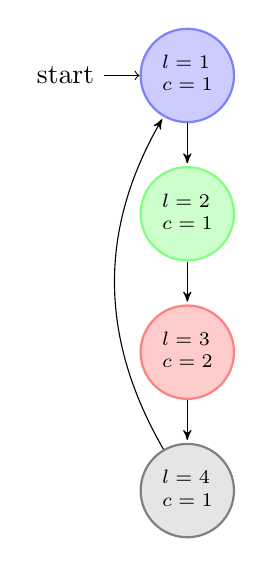
\begin{tikzpicture}
 \tikzstyle{arrow} = [->,shorten >=1pt,>=stealth'];
 \tikzstyle{place} = [circle,thick,node distance=5em,inner sep=0.05em];
 \tikzstyle{placeY} = [draw=black,fill=white];
 \tikzstyle{placeB} = [draw=blue!50,fill=blue!20];
 \tikzstyle{placeR} = [draw=red!50,fill=red!20];
 \tikzstyle{placeG} = [draw=green!50,fill=green!20];
 \tikzstyle{placeW} = [draw=black!50,fill=black!10];

 \node[place,placeB,name=i,initial]     
                                        {
					 \scriptsize
                                         $
					   \begin{array}{l}
					    l=1 \\
					    c=1
					   \end{array}
					 $};
 \node[place,placeG,name=w,below of=i]  
                                        {
					 \scriptsize
                                         $
					   \begin{array}{l}
					    l=2 \\
					    c=1
					   \end{array}
					 $};
 \node[place,placeR,name=c,below of=w] 
                                        {
					 \scriptsize
                                         $
					   \begin{array}{l}
					    l=3 \\
					    c=2
					   \end{array}
					 $};
 \node[place,placeW,name=e,below of=c]
                                        {
					 \scriptsize
                                         $
					   \begin{array}{l}
					    l=4 \\
					    c=1
					   \end{array}
					 $};

 \path (i) edge [arrow] node [above] {} (w);
 \path (w) edge [arrow] node [above] {} (c);
 \path (c) edge [arrow] node [above] {} (e);
 \path (e) edge [arrow, bend left] node [below] {} (i);
\end{tikzpicture}
\endpgfgraphicnamed

\end{document}


